\documentclass{article}

\usepackage{graphicx}
\usepackage{tikz}
\usepackage{tikzsymbols}
\usetikzlibrary{calc,patterns,shapes.geometric}
\pagestyle{empty}
\usepackage[margin=0pt]{geometry}
\geometry{papersize={14in,12in}}

\def\centerarc[#1](#2)(#3:#4:#5){\draw[#1] ($(#2)+({#5*cos(#3)},{#5*sin(#3)})$) arc (#3:#4:#5);}

\begin{document}
	\begin{figure}
		\centering
		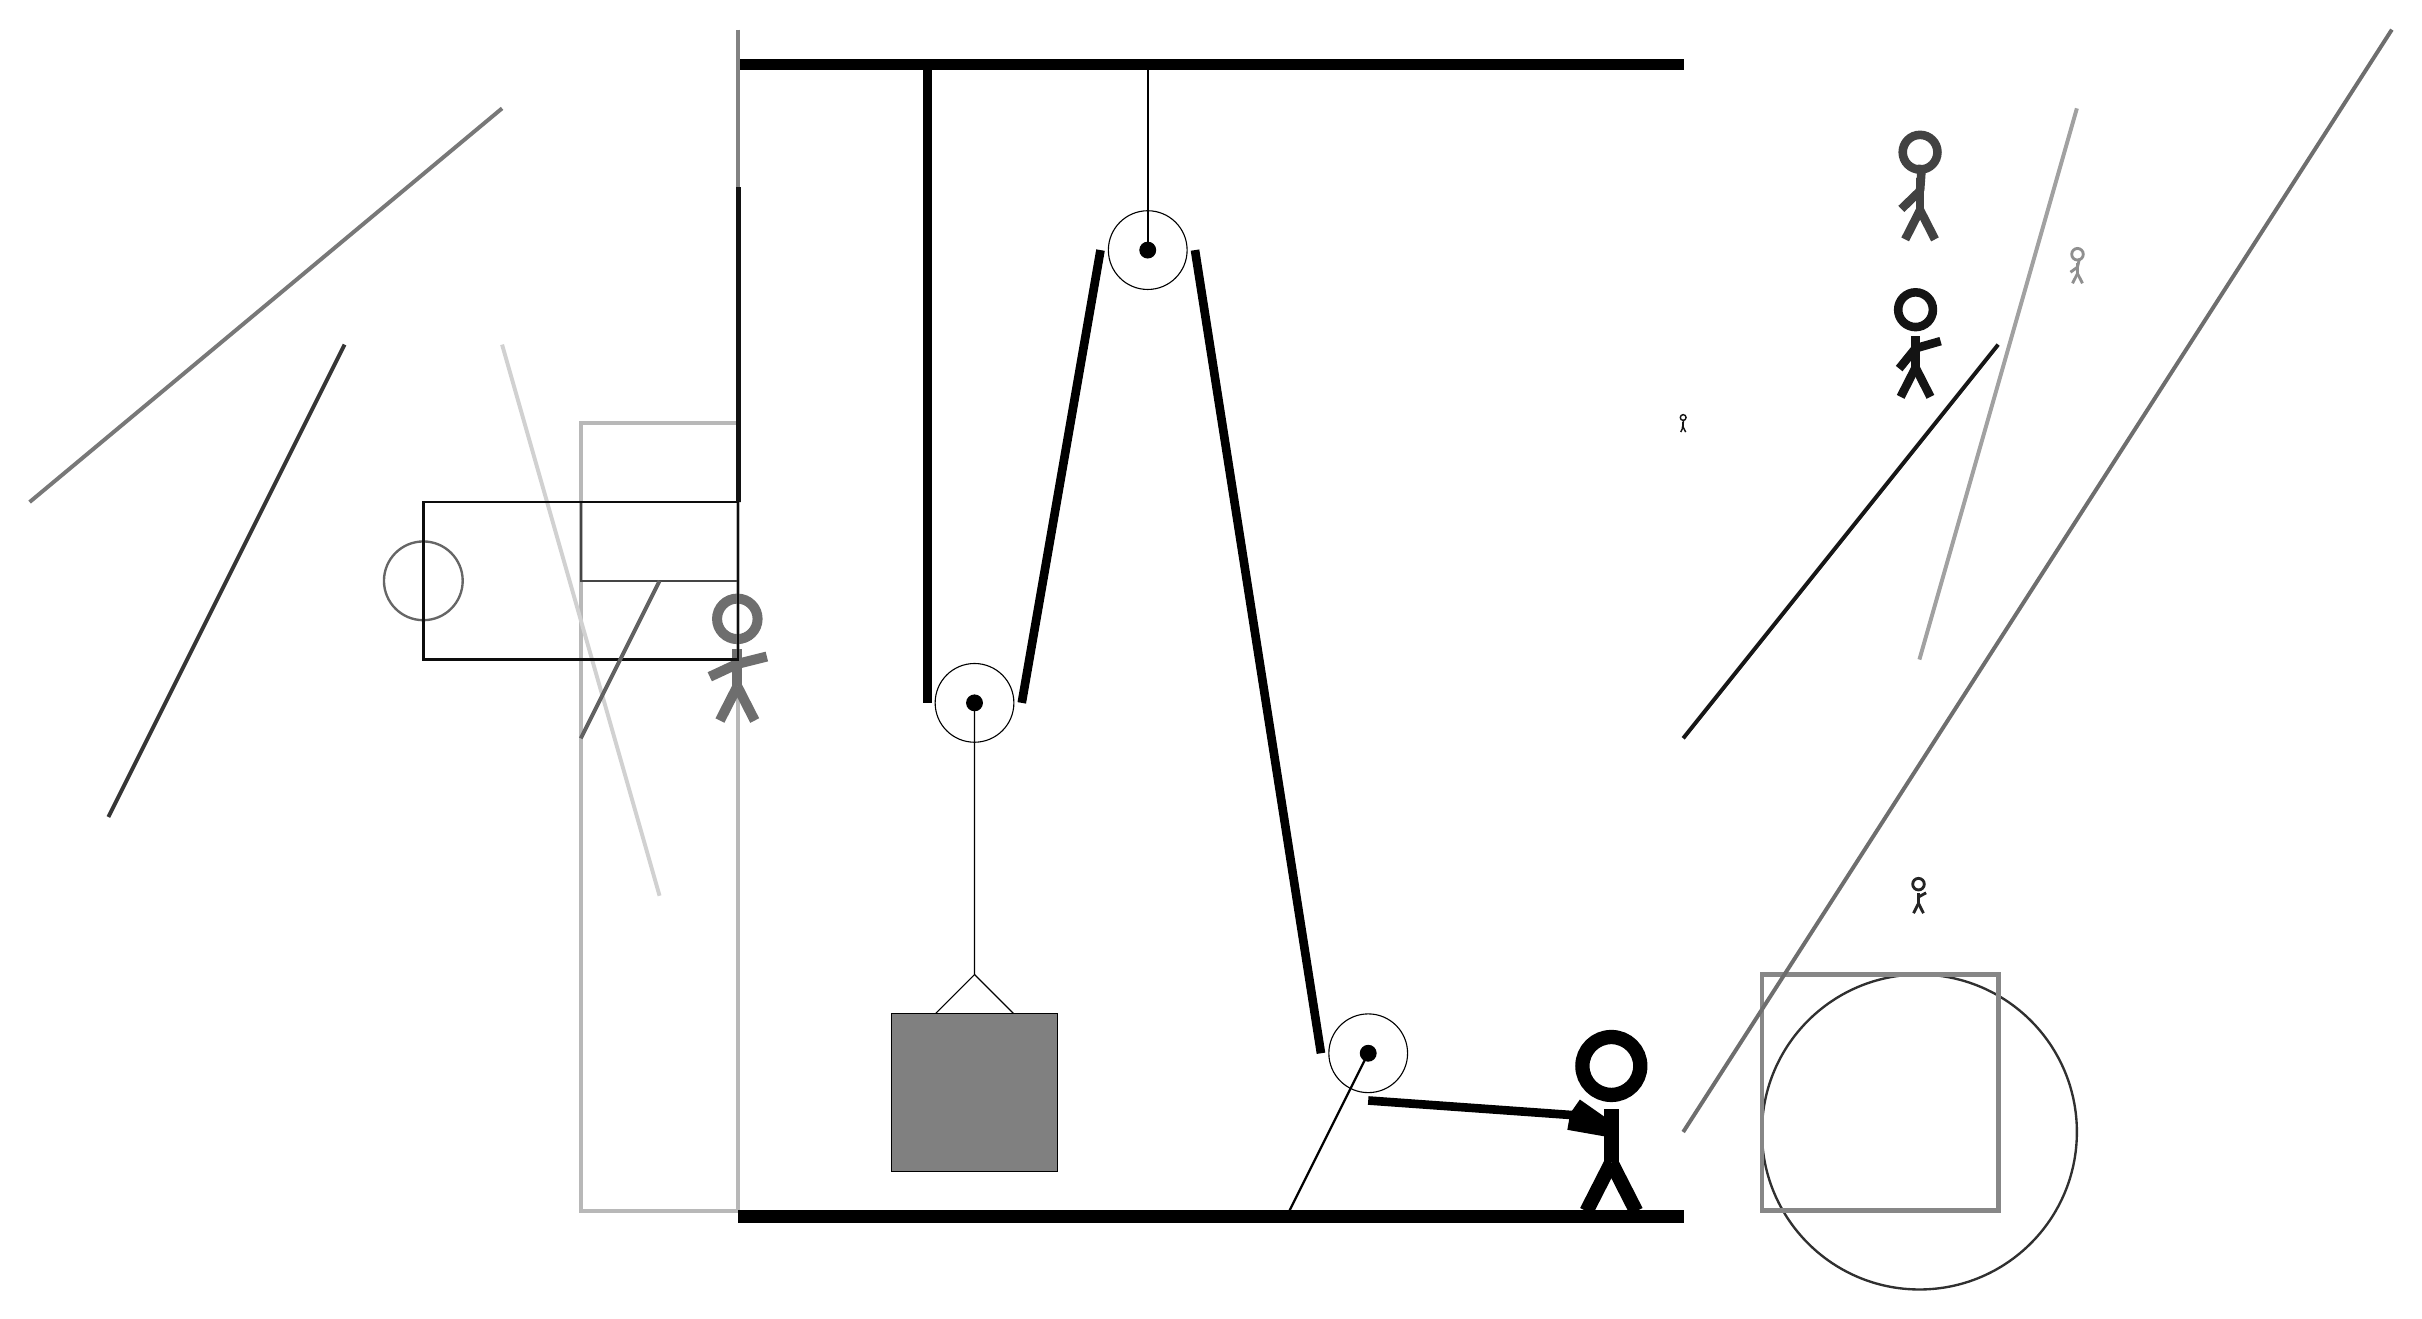
\begin{tikzpicture}
			%%%%% START %%%%%
			
			\draw[fill=black] (-2, 11.5) rectangle (10, 11.625);
			
			\draw (3.2, 9.2) circle (0.5);
			\draw[fill=black] (3.2, 9.2) circle (0.1);
			\draw[thick] (3.2, 9.2) -- (3.2, 11.5);
			
			\draw[line width=0.5mm, color=black!37](15, 11) -- (13, 4);
			
			\draw[line width=0.5mm, color=black!49](-2, 12) -- (-2, 10);
			\draw [line width=0.3mm, color=black!81](13, -2) circle (2.0);
			\node[line width=0.2mm, color=black!86] at (13, 1) {\Strichmaxerl[2][90][29]};
			\node[line width=0.2mm, color=black!44] at (15, 9) {\Strichmaxerl[2][36][77]};
			\draw[line width=0.5mm, color=black!28] (-2, 7) rectangle (-4, -3);
			
			\draw[line width=0.6mm, color=black!47] (11, 0) rectangle (14, -3);
			
			\draw[line width=0.5mm, color=black!79](-7, 8) -- (-10, 2);
			\node[line width=0.2mm, color=black!57] at (-2, 4) {\Strichmaxerl[7][25][14]};
			\node[line width=0.2mm, color=black!74] at (13, 10) {\Strichmaxerl[6][44][86]};
			\draw[line width=0.3mm, color=black!73] (-4, 5) rectangle (-2, 6);
			
			\draw [line width=0.3mm, color=black!60](-6, 5) circle (0.5);
			\draw[line width=0.5mm, color=black!18](-5, 8) -- (-3, 1);
			
			\node[line width=0.3mm, color=black!92] at (10, 7) {\Strichmaxerl[1][78][86]};
			\draw[line width=0.3mm, color=black!95] (-2, 6) rectangle (-6, 4);
			\draw[line width=0.5mm, color=black!62](-3, 5) -- (-4, 3);
			
			\draw[line width=0.5mm, color=black!57](10, -2) -- (19, 12);
			
			\draw[line width=0.6mm, color=black!93] (-2, 10) rectangle (-2, 6);
			\draw[line width=0.5mm, color=black!91](14, 8) -- (10, 3);
			
			\node[line width=0.6mm, color=black!92] at (13, 8) {\Strichmaxerl[6][51][16]};
			\draw[line width=0.5mm, color=black!53](-5, 11) -- (-11, 6);
			
			
			\draw (6, -1) circle (0.5);
			\draw[fill=black] (6, -1) circle (0.1);
			\draw[thick] (6, -1) -- (5, -3);
			
			\draw (1, 3.45) circle (0.5);
			\draw[fill=black] (1, 3.45) circle (0.1);
			
			\draw (1, 3.45) -- (1, 0.0) -- (0.5, -0.5);
			\draw (1, 0.0) -- (1.5, -0.5);
			\draw[fill=black!50] (-0.05, -0.5) rectangle (2.05, -2.5);
			
			\draw[line width=1.1mm] (0.4, 11.5) -- (0.4, 3.45);
			\centerarc[line width=1.1mm](1, 3.45)(180:360:0.6);
			\draw[line width=1.1mm](1.6, 3.45) -- (2.6, 9.2);
			\centerarc[line width=1.1mm](3.2, 9.2)(0:180:0.6);
			\draw[line width=1.1mm](3.8, 9.2) -- (5.4, -1);
			\centerarc[line width=1.1mm](6, -1)(180:270:0.6);
			\draw[line width=1.1mm](6, -1.6) -- (8.8, -1.8);
			
			\node at (9, -1.9) {\Strichmaxerl[10][-35][170]};
			
			\draw[fill=black] (-2, -3) rectangle (10, -3.15);
			
			%%%%% END %%%%%
		\end{tikzpicture}
	\end{figure}	
\end{document}